\documentclass{article}
\usepackage[utf8]{inputenc}

\title{Lesson 5 - Computer Organization}
\author{Matt Chung}
\date{July 18 2017}
\usepackage{amsfonts}
\usepackage{ulem}
\usepackage{amsmath}
\usepackage{tikz}
\usepackage{graphicx} 
\usetikzlibrary{calc}

\begin{document}

\maketitle

\section{}
% https://tex.stackexchange.com/questions/32886/how-to-fit-a-large-figure-to-page
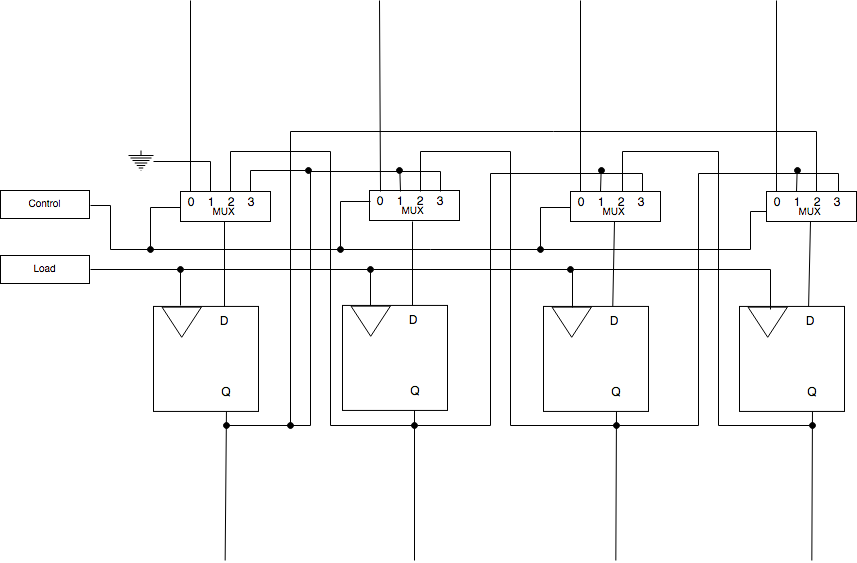
\includegraphics[width=\textwidth, height=\textheight, keepaspectratio]{q1}

\section{}
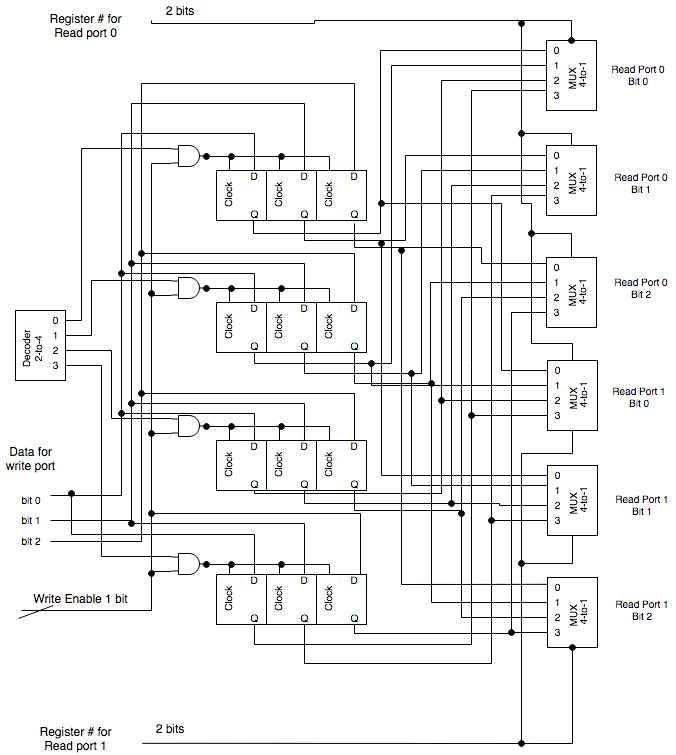
\includegraphics[width=\textwidth, height=\textheight, keepaspectratio]{lesson-5-question-2}

\section{}
Despite the drawback of requiring to be refreshed, dynamic RAM is preferred over static memory for a several reasons. To store a single bit, static memory requires four gates: (2) NOR and (2) AND gates. We can reduce the number of gates by replacing this with a capacitor (i.e. dynamic RAM), allowing us to add four times as much memory.
\section{}

Although main memory can be implemented with "register-file" design, there's a more preferred approach called "square memory." Ultimately, choosing one implementation over another boils down to one metric: effiency.  In both designs, we need two components: decoder and mux. The decoder maps the input, the memory address, to the right register/memory; the mux maps the output to the right ports. But for the "register-file" design, the number of gates for decoders and mux grow exponentially as we increase the number of bits (i.e. memory address). We can reduce these number of gates with a "square memory" design that allows us to reduce the number gates for both the decoder and the mux.

We reduce the number of gates for the decoder by replacing the large decoder with two smaller decoders. And although we can eliminate the mux, we must replace them with a set of tri-state buffers.

\section{}
\textit{Suppose we are implementing 1G $\times$ 8 (1 G registers, each with 8-bits)}

\subsection{}
\textit{How many and what type of decoder?}

The purpose of a decoder is to toggle the inputs (e.g. memory address) to the correct outputs. With a total of $2^{30}$ memory addresses, we need the following control bits: 30 bits; this is defined as a \textbf{30-to-$2^{30}$ decoder}

\subsection{}
\textit{How many total gates needed for these decoders (assume 9 input limit for both AND and OR gates)}

If we refer back to assignment 4, we know that for every decoder output requires a single AND gate. Therefore, we would need $2^30$-input AND gates; but since each input AND gate is limited to 9 inputs, we'll need to construct the AND gate from four AND gates. Therefore, the total number of AND gates required can be calculated as: $2^30 * 4$

\subsection{}
\textit{How many and what type of MUX?}

To answer this question, we need two pieces of information: the number of registers and the number of bits.  The number of registers determines the \textit{type} of MUX; the number of bits, the number of MUX.  Since we have $2^{30}-1$ registers, we'll need a $2^{30}-to-1 mux$. And since we have 8-bits, we'll need 8 of these MUX.

\subsection{}
\textit{How many total gates for MUX (assume 9 input limit for both AND and OR gates)?}


\end{document}